\documentclass[../_main/handlingar.tex]{subfiles}

\begin{document}
\motion{Renovering av Biljard}

Biljard har under min tid här på E-sektionen varit i ett stort behov av renovering eller
åtminstone en uppfräschning. Biljardbordet lutar och ger ifrån sig skrämmande ljud vid
belastning, darttavlan håller på att falla sönder, sofforna är sunkiga, det läggs alldeles för
mycket skräp där som blockerar nödutgångar med jämna mellarum och det finns en
TV-skärm som hade kunnat bytas ut till det bättre. Jag hade då velat byta ut biljardbordet
mot ett bättre, slänga allt skräp, byta ut soffor mot 3 st barbord + stolar, köpa in en ordentlig
darttavla, köpa in en ny skärm samt måla om och göra biljard till det pubrum det aspirerar till
att vara. Jag skulle helst även vilja byta ut det blå skåpet men lyckades inte hitta ett liknande
skåp och ett hänglås är att föredra. Även belysningen hade kanske kunna bytas ut men det
anser jag är ett mindre problem och det kan man kanske göra i samband med en större
renovering i framtiden.

Angånde Biljardbord kan man välja 3 alternativ - Högbudget, mellanbudget och lågbudget.
Ett Biljardbord “Eagle”-komplett kostar 32000 kr och är ett hållbart alternativ men är nog i
den dyrare prisklassen. (Mått 210*118- spelyta). Ett biljardbord av varianten “Biljardai Club)
kostar 18000 och har yttermåtten 254 * 141 och är ett bra mellanklassalternativ. Det sista
bordet är ett Cambridge 7-bord som kostar 6500 kr och är något mindre med en spelyta på
190*95 och 213x118 som yttermått. Detta står i kontrast mot dagens bord som har yttermått
på ca 255* 140. Det kanske skulle vara en fördel att ha ett något mindre bord för att frigöra
mer yta men gör man sig av med sofforna på ena sidan så ser jag inte problemet i att ha ett
bord lika stort som det som finns nu. Värt att tillägga är att alla tillbehör kommer till ett nytt
biljardbord och således får man två nya köer också vilket är välbehövligt. Jag skulle
rekommendera att vi köper in det bord som ligger i mellanklassbudget och är av samma
mått. Det är ett hållbart och förhållandevis prisvärt alternativ. Det dyra är i min mening
bortslösat på hobbyspel och det billiga bordets kvalitet är osäker.

Angående övrigt material - Tre bord med två tillhörande stolar vardera. Borden är 70*70cm
och är av modell Barbord Bianca för 1595krst. Stolarna är av modell atlantic och kostar
900kr st. Darttavlan som bör köpas in är av modell Unicorn Eclipse Pro och kostar 499 kr.
Sen behöver tre st färgburkar i svart, vinröd och vit färg köpas in till en budget av 300 kr st.
Tv-skärmen kan vara valfri fungerande 32-tums Tv-skärm till en maxkostnad av 2000 kr.

Planlösningen i min mening om det här genomförs skulle då bli som vackert illustrerat
nedan. Biljardbordet kan flyttas närmare väggen och frigöra mer plats till 3 bord med två
stolar vardera och göra biljard till ett riktigt härligt ställe att vistas på.


\begin{center}
    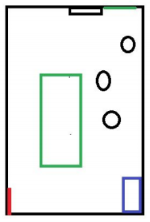
\includegraphics[width=4cm]{biljard.jpg}
\end{center}

\newpage

Äntligen är vi framme vid mitt slutgilitga yrkande. Jag yrkar

    \begin{attsatser}
       \att slänga ut allt skräp ur biljard,
       \att ersätta sofforna med tre bord av modell bianca och 6 barstolar av modell atlantic,
       \att byta ut det nuvarande biljardbordet mot ett av modell Biljardai Club,
       \att att ersätta den nuvarande darttavlan med en av modell unicorn eclipse pro,
        \att byta ut den nuvarande ickefungerande TV-skärmen mot en valfri fungerande sådan,
        \att att väggarna målas om i samma färger,
        \att att budgeten sätts till 35000 kr,
        \att kostnaden belastar utrustningsfonden, samt 
        \att renoveringen sker i sommar och läggs på beslutsuppföljningen till Höstterminsmötet 2019 med undertecknad som ansvarig.

       \att inköpet läggs på beslutsuppföljningen till Hösterminsmötet 2019, med undertecknande som ansvarig.
    \end{attsatser}
    


\begin{signatures}{1}
        I sektionens tjänst
        \signature{Adam Belfrage}{Entertainer 2018}
    \end{signatures}
\end{document}



\end{document}
